\chapter{Creating Content}
\label{ch:creating_content}

\section{Creating a basic page}
In the previous chapter we learned how to create a content type. In this chapter we will learn how to create the content itself. An instance of a content type (a.k.a. a piece of content) is called a Node in Drupal. Creating content is easy, just go to Content → Add content. On this page you will see an overview of the different content types (Figure 5.1)

Figure 5.1: Add content, overview content types
We are going to add a basic page. This page will explain who we are. Go to Content → Add content → Basic page. Use the following settings:
Title: About us
Body: We are a great and fully independent American news agency sponsored by Facebook, Twitter and the Russian government.
On the right side you have several menu items. These allow you to change your posts properties. Under Menu settings add a menu link to the Main navigation (figure 5.2)

Figure 5.2: Basic page publishing options
Click Save and publish

\section{Creating a News Item}
Go to Content → Add content → News Item. Figure 5.3 shows the editing page for our news item. 

Figure 5.3: Create News item form.
This form has the fields Body, NewsTitle, Image, and News Category. These fields were added by ourselves when we created the Content Type News Item (section 4.2.4). You can see there is also a Title* field. Every Content Type always has a required Title field. There is no way to get rid of it. We will not use the NewsTitle field for now, but instead of deleting it, we will hide it in the form, as an exercise. In the meantime, we will tweak some other details of the from.
Go to: Structure → Content types → News item → Manage fields → Manage form display. Move the edit fields like in figure 5.4.

Figure 5.4: Manage form display.
Now go back to the content creation page: Content → Add content → News item. 
Fill in a title, put some text in de body, add an image and use “sports” as tag.
Click Save and publish. You should see a page like figure 5.5.

Figure 5.5: Sport news item.
We would like to change the way our news item is displayed. To do this go to: Structure → Content types → News Item → Manage display. Change it to look like figure 5.6









Figure 5.6: Manage news item display
Click Save. The news item page should look like figure 5.7

Figure 5.7: sport new item
To be honest, it looks a bit better than before but still not great. In the chapter about theming we will learn how to further change the layout by adding custom css.

\section{Review exercises}

\begin{enumerate}
    \item Add a basic page to your bitingbugs site. This page will explain why it is good to eat bugs. The title is ‘Why bugs’, the body: See file chapter5/reasonstoeatbugs.txt included in the course attachments. Add a menu link.
    
   \item	Add the recipe ‘Dry Roasted Crickets’ to your bitingbugs site.
    
    \begin{itemize}
        \item Name: Dry Roasted Crickets
        \item Ingredients: 25 - 50 live crickets
        \item Estimated time: 10 min.
        \item Directions: See file recipe\textunderscore roasted \textunderscore crickets.txt
        \item Image: See file roasted\textunderscore crickets.jpg (Alternative text: Plate of bugs)
        \item Type: snack 
    \end{itemize}

    
    \item Change it to look like figure \ref{fig:bb_recipe}
    
    \begin{figure}[h]
        \centering
        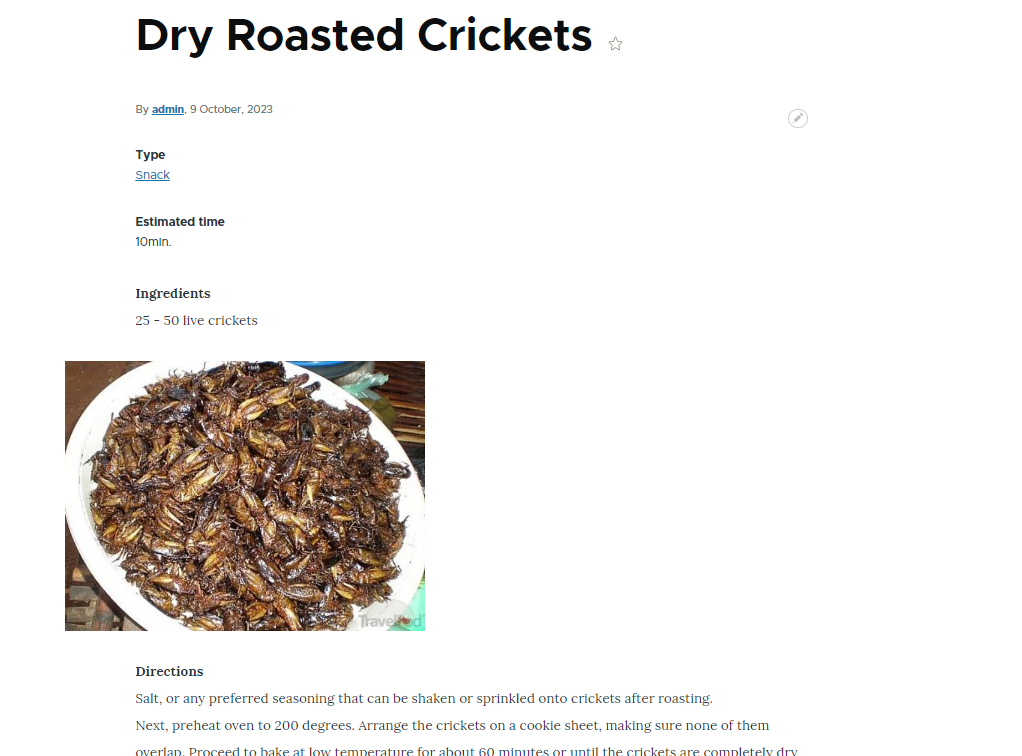
\includegraphics[width=1\linewidth]{img/ch5/bb_recipe}
        \caption{Default view of a recipe}
        \label{fig:bb_recipe}
    \end{figure}
    
   \item Go to the homepage of your site. Then, change the display settings of the recipe content type teaser display mode so it looks like figure \ref{fig:bb_recipe_teaser} Make sure that when you click the image you go to the full recipe.
    
    HINT: You can edit the image size by clicking on the gear next to the image field.
    
       \begin{figure}[h]
       \centering
       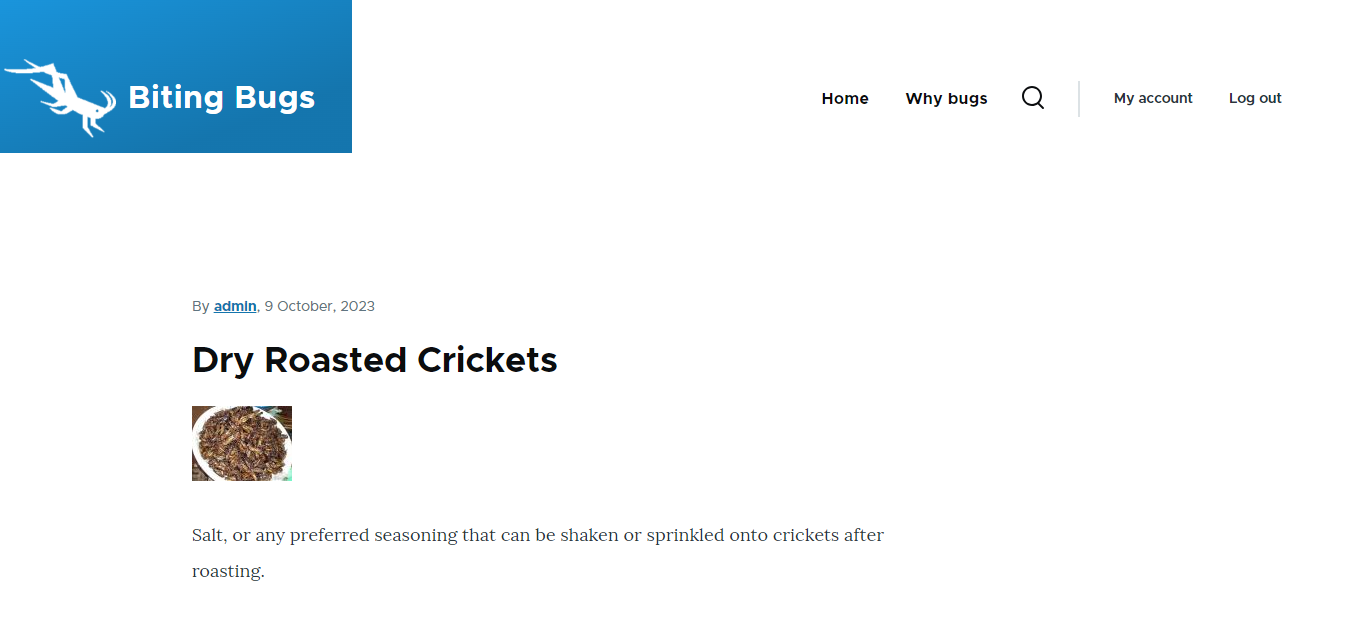
\includegraphics[width=1\linewidth]{img/ch5/bb_recipe_teaser}
       \caption{Teaser view of a recipe}
       \label{fig:bb_recipe_teaser}
   \end{figure} 
    
   \item Add three recipes to the bitingbugs site. You can find the recipes in the chapter5 resource folder: recipes\textunderscore with \textunderscore bugs.txt. Use the images: cricket-flour.jpg, cricket \textunderscore fried \textunderscore rice.jpg and cricket \textunderscore pad \textunderscore thai.jpg.
   
   \item	Logout of the bitingbugs site. On the homepage you can see a “Log in” link. Make sure the login form does not appear on the homepage, but still on all other pages. (Use Use Visibility > Pages > Hide for the listed pages) . 
    HINT: after removing the login form from the homepage you can always login by going to site hostname/<site>/web/user for example http://localhost/bb/web/user
    
    \item	Change the Recipe content type so the author information is not displayed.
    
    \item	Add a new basic page to the main menu. The basic page contains the information found in file chapter5/edible \textunderscore bugs.txt and has the title Edible bugs. (Put the bug names in bold font.) Make sure the new page appears at the right side of “Why Bugs” in the menu.
\end{enumerate}